\documentclass{../../../oss-ap12ibhl}
\usepackage{multicol}

\begin{document}
\genheader

\gentitle{15}{LIGHT AND GEOMETRIC OPTICS}

\begin{questions}
  \question In a laboratory experiment, you shine a green laser past a strand of
  hair. This produces a light and dark pattern on a screen. You notice that
  the lab group next to you has produced a similar pattern on a screen, but
  the light and dark areas are spread farther apart. Which of the following
  could cause the light and dark pattern to spread? 3
  \begin{choices}
    \choice The second group used thinner hair.
    \choice The second group is using a red laser.
    \choice The second group had the screen closer to the hair.
    \choice The second group held the laser farther from the hair.
  \end{choices}
    
  \question An observer can hear sound from around a corner but cannot see light
  from around the same corner. Which of the following helps to explain this
  phenomenon?
  \begin{choices}
    \choice Sound is a longitudinal wave, and light is an electromagnetic wave.
    \choice Sound is a mechanical wave, and light is a transverse wave.
    \choice Light travels at a speed much faster than that of sound.
    \choice Light has a much smaller wavelength than sound.
  \end{choices}
    
  \question A mirror produces an upright image one-half the height of the object
  when the object is 12 cm from the mirror's surface. What is the focal
  length of the mirror?
  \begin{choices}
    \choice\SI{-12}{\centi\metre}
    \choice\SI{-4}{\centi\metre}
    \choice\SI{4}{\centi\metre}
    \choice\SI{6}{\centi\metre}
  \end{choices}

  \question A light ray with a wavelength of $\lambda_w$ and a frequency of
  $f_w$ in water ($n=1.33$) is incident on glass ($n=1.61$). In the glass,
  the wavelength and frequency of the light is $\lambda_g$ and $f_g$. How do
  the values of wavelength and frequency of the ray of light in water compare
  to those in glass?
  \begin{choices}
    \choice $\lambda_w>\lambda_g$, and $f_w=f_g$
    \choice $\lambda_w>\lambda_g$, and $f_w>f_g$
    \choice $\lambda_w<\lambda_g$, and $f_w=f_g$
    \choice $\lambda_w<\lambda_g$, and $f_w<f_g$
  \end{choices}

  \question An optics bench is set up on a meter stick, as shown in the figure.
  The light source is a candle placed at $x_0$ . The lens is located at $x_1$.
  The screen is moved until a sharp image appears at location $x_2$. The data is
  recorded in a table, the lens is moved to a new location ($x_1$), and the
  screen is adjusted until the image is sharp again. Which of the following
  procedures will allow a student to determine the focal length of the lens?
  \cpic{.48}{meter-stick}
  \begin{choices}
    \choice Plot $x_2$ as a function of $x_0$. The focal length will be the
    vertical axis intercept.
    \choice Plot ($x_2-x_1$) as a function of ($x_0-x_1$). The focal length will
    be the vertical axis intercept.
    \choice Plot $1/x_2$ as a function of $1/x_0$. The focal length will be the
    inverse of the vertical axis intercept.
    \choice Plot $1/(x_2-x_1)$ as a function of $1/(x_0-x_1)$. The focal length
    will be the inverse of the vertical axis intercept.
  \end{choices}

  \question A laser beam passes through a prism and produces a bright dot of
  light a distance of $x$ from the prism, as shown in the figure. Which of the
  following correctly explains the change in distance as the angle
  ($\theta$) of the prism is decreased?
  \cpic{.3}{triangle}
  \begin{choices}
    \choice The distance increases because the angle on incidence increases.
    \choice The distance increases because the angle of incidence decreases.
    \choice The distance decreases because the angle on incidence increases.
    \choice The distance decreases because the angle of incidence decreases.
  \end{choices}

  \question In the human eye, the distance from the lens to the retina, on
  which the image is focused, is 20 mm. A book is held 30 cm from the eye, and
  the focal length of the eye is 16 mm. How far from the retina does the
  image form, and what lens should be used to place the image directly
  on the retina?
   
  \begin{tabular}{cll}
    & \underline{Distance of image from retina}
    & \underline{Corrective lens} \\
    (A) & 3.1 mm in front of the retina & Concave lens \\
    (B) & 3.1 mm in front of the retina & Convex lens \\
    (C) & 14 mm behind the retina & Concave lens \\
    (D) & 14 mm behind the retina & Convex lens
  \end{tabular}
  \newpage
  
% TAKEN FROM THE 2001 AP PHYSICS B EXAM FREE-RESPONSE QUESTION #4
  \uplevel{
    \cpic{.4}{glass1}
  }

  \question In an experiment a beam of red light of wavelength 675 nm in air
  passes from glass into air, as shown above. The incident and refracted angles
  are $\theta_1$ and $\theta_2$, respectively. In the experiment, angle
  $\theta_2$ is measured for various angles of incidence $\theta_1$, and the
  sines of the angles are used to obtain the line shown in the following graph.
  \cpic{.6}{graph1}
  
  \begin{parts}
    \part Assuming an index of refraction of 1.00 for air, use the graph to
    determine a value for the index of refraction of the glass for the red
    light. Explain how you obtained this value.

    \part For this red light, determine the following.
    \begin{subparts}
      \subpart The frequency in air
      \subpart The speed in glass
      \subpart The wavelength in glass
    \end{subparts}
    
    \part The index of refraction of this glass is 1.66 for violet light, which
    has wavelength 425 nm in air.
    \begin{subparts}
      \subpart Given the same incident angle $\theta_1$ , show on the ray
      diagram on the previous page how the refracted ray for the violet light
      would vary from the refracted ray already drawn for the red light.
      \subpart Sketch the graph of $\sin\theta_2$ versus $\sin\theta_1$ for the
      violet light on the figure on the previous page that shows the same graph
      already drawn for the red light.
    \end{subparts}

    \part Determine the critical angle of incidence $\theta_c$for the violet
    light in the glass in order for total internal reflection to occur.
  \end{parts}
  \newpage
  
  
  % THIS IS TAKEN FROM THE 2005 AP PHYSICS B EXAM FREE-RESPONSE QUESTION #4
  \question Your teacher gives you a slide with two closely spaced slits on it.
  She also gives you a laser with a wavelength $\lambda=\SI{632}{\nano\metre}$.
  The laboratory task that you are assigned asks you to determine the spacing
  between the slits. These slits are so close together that you cannot measure
  their spacing with a typical measuring device.
  \begin{parts}
    \part From the list below, select the additional equipment you will need to
    do your experiment by checking the line next to each item.
    \begin{multicols}{3}
      \underline{\hspace{.3in}} Meterstick\\
      \underline{\hspace{.3in}} Ruler\\
      \underline{\hspace{.3in}} Tape measure\\
      \underline{\hspace{.3in}} Light-intensity meter\\
      \columnbreak
      
      \underline{\hspace{.3in}} Large screen\\
      \underline{\hspace{.3in}} Paper\\
      \underline{\hspace{.3in}} Slide holder\\
      \underline{\hspace{.3in}} Stopwatch
    \end{multicols}
    
    \part Draw a labeled diagram of the experimental setup that you would use.
    On the diagram, use symbols to identify carefully what measurements you will
    need to make.
    \begin{center}
      \begin{tikzpicture}[scale=.45]
        \draw[thick,->](-10,0)--(10,0) node[right]{Position};
        \draw[thick,->](0,-7)--(0,7) node[right]{Position};
      \end{tikzpicture}
    \end{center}
    
    \part On the axes below, sketch a graph of intensity versus position that
    would be produced by your setup, assuming that the slits are very narrow
    compared to their separation.
  \end{parts}
  \newpage
  
  % THIS IS TAKEN FROM THE 2014 AP PHYSICS B EXAM FREE-RESPONSE QUESTION #7
  \uplevel{
    \centering
    \pic{.35}{film1}
    
    \underline{Note:} Figure not drawn to scale.
  }
  \question A thin layer of transparent oil is placed on top of a transparent
  plate. The oil film is then illuminated by white light shining onto the oil's
  surface, as shown in the figure above. To an observer standing right next to
  the light source and looking straight down on the oil film, the oil film
  appears green, corresponding to a wavelength of 520 nm in air. The oil has an
  index of refraction of 1.52.
  \begin{parts}
    \part Determine the frequency of the green light in the air.
    \part Determine the frequency of the green light in the oil film.
    \part Calculate the wavelength of the green light in the oil film.
    \part The oil film thickness is half of the wavelength you found in part
    (c). Is the index of refraction of the plate greater than, less than, or
    equal to that of the oil? Justify your answer.

    \uplevel{
      \centering
      \pic{.7}{film2}
      
      \underline{Note:} Figure not drawn to scale.
    }
    \part As the observer starts moving to the right away from the light source,
    as shown in the figures above, the film appears to change color. Describe
    the color change and give an explanation for this phenomenon.
  \end{parts}
  \newpage

  % THIS IS TAKEN FROM THE 2008 AP PHYSICS B EXAM FREE-RESPONSE QUESTION #6
  \uplevel{
    \cpic{.8}{converging-mirror}
  }
  
  \question The figure above shows a converging mirror, its focal point $F$, its
  center of curvature $C$, and an object represented by the solid arrow.
  \begin{parts}
    \part On the figure above, draw a ray diagram showing at least two incident
    rays and the image formed by them.
    \part Is the image real or virtual? Justify your answer.
    \part The focal length of this mirror is \SI{6.}{\centi\metre}, and the
    object is located \SI{8.}{\centi\metre} away from the mirror. Calculate the
    position of the image formed by the mirror. (Do NOT simply measure your ray
    diagram.)
    \part Suppose that the converging mirror is replaced by a diverging mirror
    with the same radius of curvature that is the same distance from the
    object, as shown below.
    \cpic{.8}{diverging-mirror}
    For this mirror, how does the size of the image compare with that of the
    object? Justify your answer.

    \vspace{.15in}
    \underline{\hspace{.4in}} Larger than the object\hspace{.3in}
    \underline{\hspace{.4in}} Smaller than the object\hspace{.3in}
    \underline{\hspace{.4in}} The same size as the object
  \end{parts}
  \newpage

  % THIS IS TAKEN FROM THE 2010 AP PHYSICS B EXAM FREE-RESPONSE QUESTION #5
  \uplevel{
    \centering
    \pic{.4}{prism}
    
    \underline{Note:} Figure not drawn to scale.
  }
  \question As shown above, a beam of red light of wavelength
  \SI{6.65e-7}{\metre} in air is incident on a glass prism at an angle
  $\theta_1$ with the normal. The glass has index of refraction $n=1.65$ for
  the red light. When $\theta_1=\ang{40}$, the beam emerges on the other side
  of the prism at an angle $\theta_4=\ang{84}$.
  \begin{parts}
    \part Calculate the angle of refraction $\theta_2$ at the left side of the
    prism.
    
    \part Using the same prism, describe a change to the setup that would result
    in total internal reflection of the beam at the right side of the prism.
    Justify your answer.
    
    \part The incident beam is now perpendicular to the surface. The glass is
    coated with a thin film that has an index of refraction $n_f = 1.38$ to
    reduce the partial reflection of the beam at this angle.
    \begin{subparts}
      \subpart Calculate the wavelength of the red light in the film.
      \subpart Calculate the minimum thickness of the film for which the
      intensity of the reflected red ray is near zero.
    \end{subparts}
  \end{parts}
  \newpage

  % THIS IS TAKEN FROM THE 2006 AP PHYSICS B EXAM FREE-RESPONSE QUESTION #4
  \question A student performs an experiment to determine the index of
  refraction $n$ of a rectangular glass slab in air. She is asked to use a
  laser beam to measure angles of incidence $\theta_i$ in air and corresponding
  angles of refraction $\theta_r$ in glass. The measurements of the angles for
  five trials are given in the table below.
  \begin{center}
    \bgroup
    \def\arraystretch{1.7}
    \begin{tabular}{|c|c|c|p{1in}|p{1in}|}
      \hline
      Trial & $\theta_i$ & $\theta_r$ & & \\ \hline
      \hspace{.2in}1\hspace{.2in} & \hspace{.2in}\ang{30}\hspace{.2in} &
      \hspace{.2in}\ang{20}\hspace{.2in} & & \\ \hline
      2 & \ang{40} & \ang{27} & & \\ \hline
      3 & \ang{50} & \ang{32} & & \\ \hline
      4 & \ang{60} & \ang{37} & & \\ \hline
      5 & \ang{70} & \ang{40} & & \\ \hline
    \end{tabular}
    \egroup
  \end{center}
  \begin{parts}
    \part Complete the last two columns in the table by calculating the
    quantities that need to be graphed to provide a linear relationship from
    which the index of refraction can be determined. Label the top of each
    column.
    
    \part On the grid below, plot the quantities calculated in (a) and draw an
    appropriate graph from which the index of refraction can be determined.
    Label the axes.
    \begin{center}
      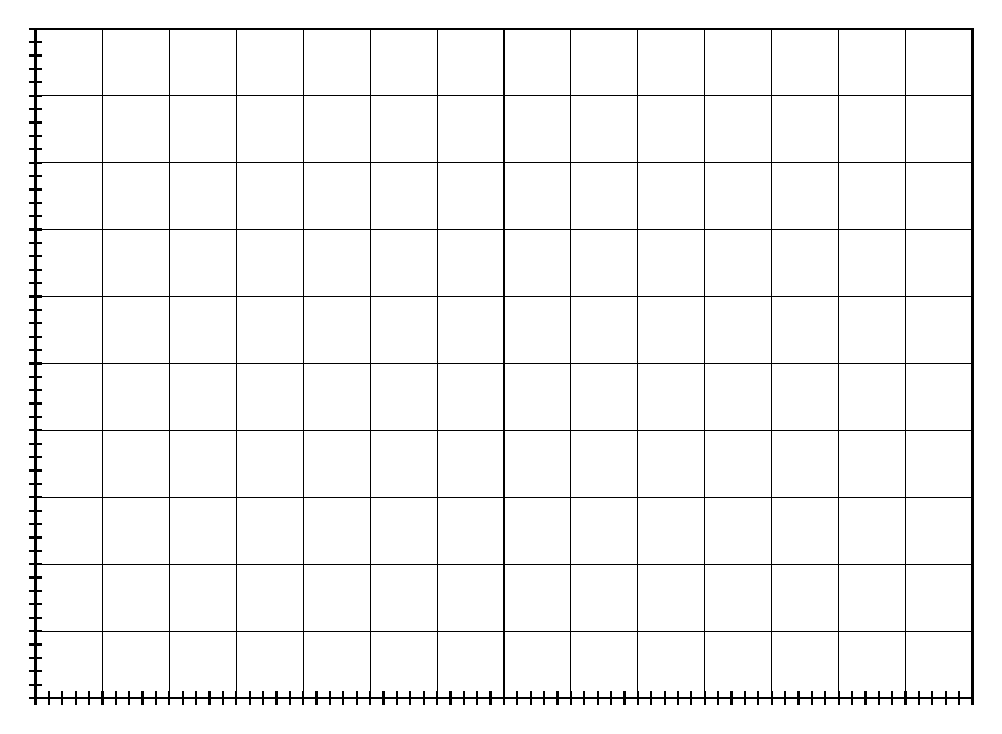
\begin{tikzpicture}[scale=.85]
        \draw[thick](0,0) rectangle(14,10);
        \draw(0,0) grid(14,10);
        \foreach\x in {0,.2,.4,...,14}\draw[thick](\x,-.1)--(\x,.1);
        \foreach\y in {0,.2,.4,...,10}\draw[thick](-.1,\y)--(.1,\y);
      \end{tikzpicture}
    \end{center}

    \part Using the graph, calculate the index of refraction of the glass slab.
    \begin{center}
      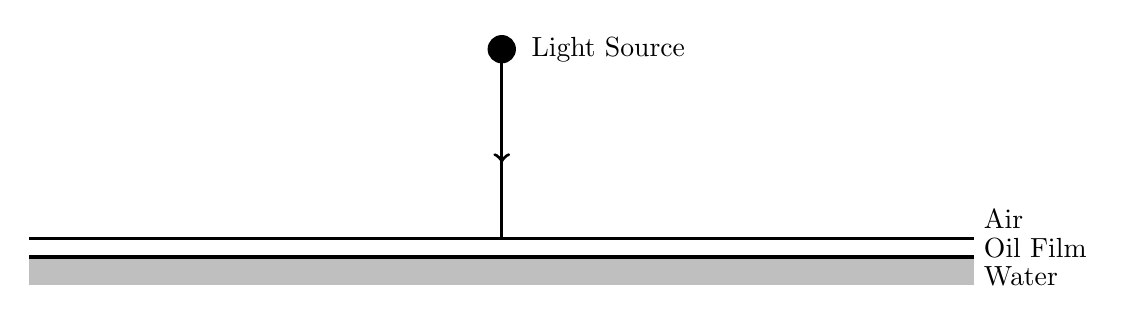
\begin{tikzpicture}[scale=1.2]
        \fill(5,2) circle(.15) node[right]{\hspace{.1in}Light Source};
        \draw[very thick](5,2)--(5,0);
        \draw[very thick,->](5,2)--(5,.8);
        \draw[very thick](0,0)--(10,0);
        \fill[gray!50](0,-.2) rectangle(10,-.5);
        \draw[very thick](0,-.2)--(10,-.2);
        \node[right] at (10,.2) {Air};
        \node[right] at (10,-.1){Oil Film};
      \node at (10,-.4)[right]{Water};
      \end{tikzpicture}
    \end{center}
    \uplevel{
      The student is also asked to determine the thickness of a film of oil
      ($n=1.43$) on the surface of water ($n=1.33$). Light from a variable
      wavelength source is incident vertically onto the oil film as shown above.
      The student measures a maximum in the intensity of the reflected light
      when the incident light has a wavelength of \SI{600}{\nano\metre}.
    }

    \part At which of the two interfaces does the light undergo a \ang{180}
    phase change on reflection?

    \vspace{.1in}
    \underline{\hspace{.4in}} The air-oil interface only\hspace{.3in}
    \underline{\hspace{.4in}} The oil-water interface only\hspace{.3in}
    \underline{\hspace{.4in}} Both interfaces\hspace{.3in}\\
    \underline{\hspace{.4in}} Neither interface
    \vspace{.1in}
    
    \part Calculate the minimum possible thickness of the oil film.
  \end{parts}
  \newpage
  
  % TAKEN FROM THE 2015 AP PHYSICS 2 EXAM FREE-RESPONSE QUESTION #1
  \uplevel{
    \cpic{.5}{drinkingglass1}
  }
  \question The figure above shows a cross section of a drinking glass (index
  of refraction 1.52) filled with a thin layer of liquid (index of refraction
  1.33). The bottom corners of the glass are circular arcs, with the bottom
  right arc centered at point $O$. A monochromatic light source placed to the
  right of point $P$ shines a beam aimed at point $O$ at an angle of incidence
  $\theta$. The flat bottom surface of the glass containing point $P$ is
  frosted so that bright spots appear where light from the beam strikes the
  bottom surface and does not reflect. When $\theta=\theta_1$, two bright
  spots appear on the bottom surface of the glass. The spot closer to point $P$
  will be referred to as $X$; the spot farther from $P$ will be referred to as
  $Y$. The location of spot $X$ and that of spot $Y$ both change as $\theta$ is
  increased.
  \begin{parts}
    \part In a coherent paragraph-length answer, describe the processes
    involved in the formation of spots $X$ and $Y$ when $\theta=\theta_1$.
    Include an explanation of why spot $Y$ is located farther from point $P$
    than spot $X$ is and what factors affect the brightness of the spots.

    \part When $\theta$ is increased to $\theta_2$, one of the spots becomes
    brighter than it was before, due to total internal reflection.
    \begin{subparts}
      \subpart On the figure below, draw a ray diagram that clearly and
      accurately shows the formation of spots $X$ and $Y$ when
      $\theta=\theta_2$.
      \uplevel{
        \cpic{.5}{drinkingglass2}
      }
      
      \subpart Which spot, $X$ or $Y$, becomes brighter than it was before due
      to total internal reflection? Explain your reasoning.
    \end{subparts}
    \part When $\theta$ is further increased to $\theta_3$, one of the spots
    disappears entirely.
    \begin{subparts}
      \subpart On the figure below, draw a ray diagram that clearly and
      accurately shows the formation of the remaining spot, $X$ or $Y$, when
      $\theta=\theta_3$.
      \uplevel{
        \cpic{.5}{drinkingglass3}
      }
      \subpart Indicate which spot, $X$ or $Y$, disappears. Explain your
      reasoning in terms of total internal reflection.
    \end{subparts}
  \end{parts}
\end{questions}
\end{document}
